\subsection{Упражнение 1}

Скачайте с сайта http://freesound.org , включающий музыку, речь или иные звуки, имеющие четко выраженную высоту. Выделите примерно полусекундный сегмент, в котором высота постоянна. Вычислите и распечатайте спектр выбранного сегмента. Как связаны тембр звука и гармоническая структура, видимая в спектре?


\noindent Используйте high\_pass, low\_pass, и band\_stop для фильтрациитех или иных гармоник. Затем преобразуйте спектры обратно в сигнал и прослушайте его. Как звук соотносится с изменениями, сделанными в спектре?
    

Загрузим выбранный звук пианино

\begin{lstlisting}[language=Python]
if not os.path.exists('440931__xhale303__piano-loop-1.wav'):
  !wget https://github.com/hotnotHD/Telecom/raw/main/440931__xhale303__piano-loop-1.wav
wave = read_wave('440931__xhale303__piano-loop-1.wav')

wave.make_audio()
\end{lstlisting}

Построим график wave
\begin{lstlisting}[language=Python]
wave.plot()
decorate(xlabel='Time (s)')
\end{lstlisting}

\begin{figure}[H]
	\begin{center}
		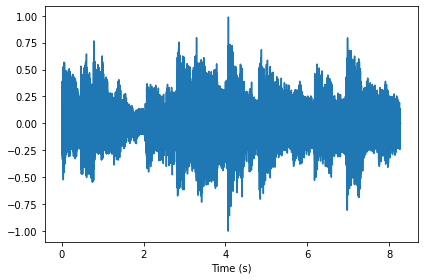
\includegraphics[scale=1]{fig/lab01/lab01_01.png}
		\caption{График всего звука}
	\end{center}
\end{figure}

Выделяем полусекундный сегмент
\begin{lstlisting}[language=Python]
segment = wave.segment(start=3, duration=0.5)
segment.make_audio()

segment.plot()
decorate(xlabel='Time (s)')
\end{lstlisting}

\begin{figure}[H]
	\begin{center}
		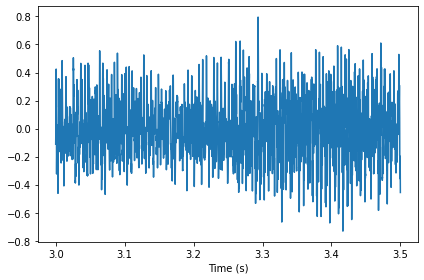
\includegraphics[scale=1]{fig/lab01/lab01_02.png}
		\caption{График сегмента звука}
	\end{center}
\end{figure}

Спектр сегмента
\begin{lstlisting}[language=Python]
spectrum = segment.make_spectrum()
spectrum.plot(high=6000)
decorate(xlabel='Frequency (Hz)')
\end{lstlisting}

\begin{figure}[H]
	\begin{center}
		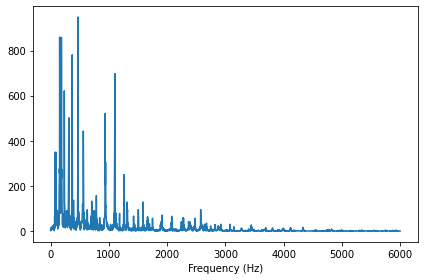
\includegraphics[scale=1]{fig/lab01/lab01_03.png}
		\caption{Спектр сегмента звука}
	\end{center}
\end{figure}

Применим функции фильтрации

Убираем частоты ниже 500
\begin{lstlisting}[language=Python]
spectrum.high_pass(500)
spectrum.plot(high=6000)
decorate(xlabel='Frequency (Hz)')
\end{lstlisting}

\begin{figure}[H]
	\begin{center}
		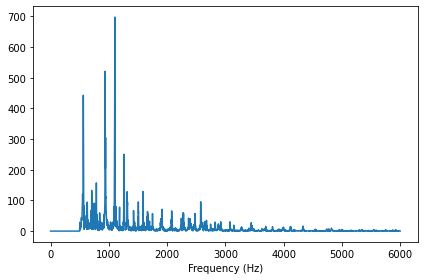
\includegraphics[scale=1]{fig/lab01/lab01_04.png}
		\caption{График частот без тех, что ниже 500}
	\end{center}
\end{figure}

Уберем частоты выше 2000
\begin{lstlisting}[language=Python]
spectrum.low_pass(2000)
spectrum.plot(high=6000)
decorate(xlabel='Frequency (Hz)')
\end{lstlisting}

\begin{figure}[H]
	\begin{center}
		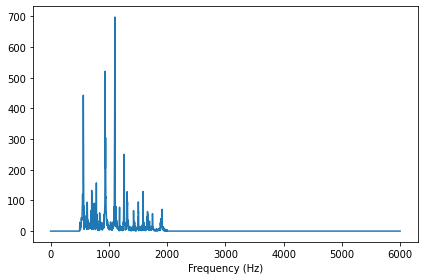
\includegraphics[scale=1]{fig/lab01/lab01_05.png}
		\caption{График частот без тех, что выше 2000}
	\end{center}
\end{figure}

Убираем частоты в срезе
\begin{lstlisting}[language=Python]
spectrum.band_stop(1100, 2500)
spectrum.plot(high=6000)
decorate(xlabel='Frequency (Hz)')
\end{lstlisting}

\begin{figure}[H]
	\begin{center}
		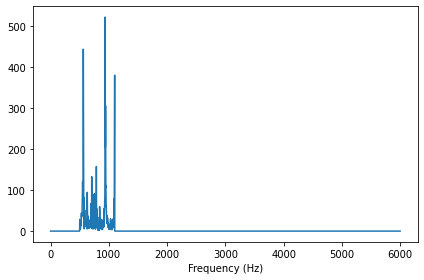
\includegraphics[scale=1]{fig/lab01/lab01_06.png}
		\caption{График частот после применения ФПЗ}
	\end{center}
\end{figure}

Переведем из спектра в волну
\begin{lstlisting}[language=Python]
test = spectrum.make_wave()
test.plot()
decorate(xlabel='Time (s)')
\end{lstlisting}

\begin{figure}[H]
	\begin{center}
		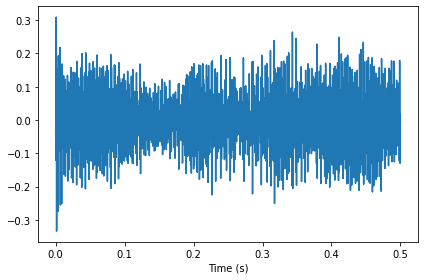
\includegraphics[scale=1]{fig/lab01/lab01_07.png}
		\caption{График преобразованного сигнала}
	\end{center}
\end{figure}

Проведем сравнение изначального среза и отфильтрованного

Изначальный срез
\begin{lstlisting}[language=Python]
segment.make_audio()
\end{lstlisting}

Отфильтрованный срез
\begin{lstlisting}[language=Python]
wave2.make_audio()
\end{lstlisting}

В итоге получаем довольно "плоский" звук, лишенный объема.


\subsection{Упражнение 2}

Создайте сложный сигнал из объектов SinSignal и CosSignal, суммируя их. Обработайте сигнал для получения wave и прослушайте его. Вычислите Spectrum и распечатайте. Что произойдёт при добавлении частотных компонент, не кратных основным?

Создадим сложный сигнал из SinSignal и CosSignal
\begin{lstlisting}[language=Python]
cos_sig = CosSignal(freq=103, amp=1.0, offset=0)
sin_sig = SinSignal(freq=206, amp=0.8, offset=0)
cos_sig2 = CosSignal(freq=412, amp=0.3, offset=0)
m_sig = cos_sig + sin_sig + cos_sig2

Построим график суммы
\begin{lstlisting}[language=Python]
m_sig.plot()

\end{lstlisting}
\begin{figure}[H]
	\begin{center}
		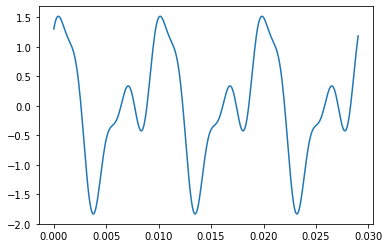
\includegraphics[scale=1]{fig/lab01/lab01_08.png}
		\caption{Графиксуммы сигналов}
	\end{center}
\end{figure}

Сделаем wave и послушаем
\begin{lstlisting}[language=Python]
wave = m_sig.make_wave()

wave.make_audio()
\end{lstlisting}

Спектр
\begin{lstlisting}[language=Python]
spectrum = wave.make_spectrum()
spectrum.plot()
\end{lstlisting}

\begin{figure}[H]
	\begin{center}
		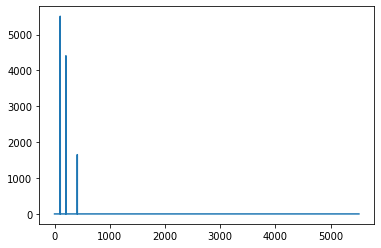
\includegraphics[scale=1]{fig/lab01/lab01_09.png}
		\caption{Спектр сигнала}
	\end{center}
\end{figure}

Добавим к этой волне ещё частотный компонент, не кратный основным
\begin{lstlisting}[language=Python]
wave2 = (m_sig + SinSignal(freq=250, amp=0.5, offset=0)).make_wave()
wave2.make_audio()

wave2.make_spectrum().plot()
\end{lstlisting}

\begin{figure}[H]
	\begin{center}
		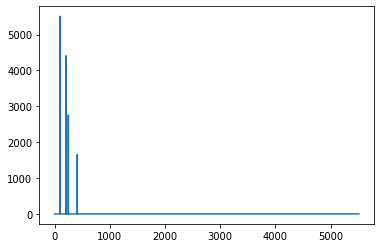
\includegraphics[scale=1]{fig/lab01/lab01_10.png}
		\caption{График после добавления частотного компонента}
	\end{center}
\end{figure}

Звук перестал быть однотонным, появился "дребезг"


\subsection{Упражнение 3}

Напишите функцию strech, берущую wave и коэффицент изменения. Она должна ускорять или замедлять сигнал изменением ts и framerate.

Создадим функцию stretch, которая будет замедлять или ускорять сигнал в зависимости от коэффициента измнения
\begin{lstlisting}[language=Python]
def stretch(wave, k):
  wave.ts *= k
  wave.framerate /= k
  
wave = read_wave('440931__xhale303__piano-loop-1.wav')
wave.make_audio()
\end{lstlisting}

Проверим функцию
\begin{lstlisting}[language=Python]
wave2 = wave
stretch(wave2, 2)
wave2.make_audio()
\end{lstlisting}

Звук замедлился в 2 раза

\subsection{Вывод}
В ходе данной работы было выполнено знакомство с основыми понятиями при работе со звуками и сигналами. При помощи библиотеки thinkDSP открывается множество возможностей по взаимодействию с сингалами, таких как их созданию, так и для их обработки